\documentclass{article}

\usepackage{float}
\restylefloat{table}

\usepackage{booktabs}
\usepackage{pgf}
\usepackage{graphicx}
\graphicspath{ {./images/} }

\title{Team Contributions: POC\\\progname}

\author{\authname}

\date{}

%% Comments

\usepackage{color}

\newif\ifcomments\commentstrue %displays comments
%\newif\ifcomments\commentsfalse %so that comments do not display

\ifcomments
\newcommand{\authornote}[3]{\textcolor{#1}{[#3 ---#2]}}
\newcommand{\todo}[1]{\textcolor{red}{[TODO: #1]}}
\else
\newcommand{\authornote}[3]{}
\newcommand{\todo}[1]{}
\fi

\newcommand{\wss}[1]{\authornote{blue}{SS}{#1}} 
\newcommand{\plt}[1]{\authornote{magenta}{TPLT}{#1}} %For explanation of the template
\newcommand{\an}[1]{\authornote{cyan}{Author}{#1}}

%% Common Parts

\newcommand{\progname}{SFWRENG 4G06} % PUT YOUR PROGRAM NAME HERE
\newcommand{\authname}{Team 9, dice\_devs
\\ John Popovici
\\ Nigel Moses
\\ Naishan Guo
\\ Hemraj Bhatt
\\ Isaac Giles} % AUTHOR NAMES                  

\usepackage{hyperref}
    \hypersetup{colorlinks=true, linkcolor=blue, citecolor=blue, filecolor=blue,
                urlcolor=blue, unicode=false}
    \urlstyle{same}
                                


\begin{document}

\maketitle

This document summarizes the contributions of each team member up to the POC
Demo.  The time period of interest is the time between the beginning of the term
and the POC demo.

Numbers for all sections as of start of 2024-11-24.

\newpage
\section{Demo Plans}

\noindent The team will demonstrate the following key components of the system during the POC demonstration. 

\begin{enumerate}
    \item \textbf{Game Setup and Customization:}
    \begin{itemize}
        \item Demonstrate how users can set up a new local area network multiplayer game.
        \item Showcase customization of gameplay attributes, such as adjusting the number of dice and player health.
        \item Through this, the modularity of the system will be displayed.
    \end{itemize}
    
    \item \textbf{Gameplay Mechanics:}
    \begin{itemize}
        \item Conduct a walkthrough of a round of gameplay, highlighting how players reroll the dice and accumulate points.
        \item Explain the scoring rules and demonstrate how player points are added.
        \item This will showcase the basic game flow.
    \end{itemize}
    
    \item \textbf{Game State and Progression:}
    \begin{itemize}
        \item Showcase how the game state is saved, i.e. how the game tracks and displays each player's current dice and hand points.
        \item Demonstrate the endgame conditions, illustrating what happens when all rounds are played and points are tallied.
        \item This will show how the system preserves game data.
    \end{itemize}
    
    \item \textbf{Multiplayer Mode:}
    \begin{itemize}
        \item Demonstrate how players take turns simultaneously and show the tracking of player dice for both players.
        \item This will highlight how data is synchronized between both players and how game integrity is preserved.
    \end{itemize}
    
    \item \textbf{Error Handling and Edge Cases:}
    \begin{itemize}
        \item Showcase implemented safeguards, such as preventing invalid moves and handling unexpected inputs through demonstrating typical game actions.
        \item Demonstrate the system's response in case of such scenarios.
        \item This will showcase the rigidity and stability of the system.
    \end{itemize}
\end{enumerate}



\newpage
\section{Meeting and Lecture Attendance}

% \wss{For each team member how many team meetings have they attended over the time period of interest.  This number should be determined from the meeting issues in the team's repo.  The first entry in the table should be the total number of team meetings held by the team.}

% \wss{For each team member how many supervisor/stakeholder team meetings have they attended over the time period of interest.  This number should be determined from the supervisor meeting issues in the team's repo.  The first entry in the table should be the total number of supervisor and team meetings held by the team.  If there is no supervisor, there will usually be meetings with stakeholders (potential users) that can serve a similar purpose.}

% \wss{For each team member how many lectures have they attended over the time period of interest.  This number should be determined from the lecture issues in the team's repo.  The first entry in the table should be the total number of lectures since the beginning of the term.}

% \wss{For each team member how many of the informal document discussion meetings with the TA were attended over the time period of interest.}

\begin{table}[H]
\centering
\begin{tabular}{lllll}
\toprule
\textbf{ } & \textbf{Team} & \textbf{Supervisor} & \textbf{ } & \textbf{TA}\\
\textbf{Student} & \textbf{Meetings} & \textbf{Meetings} & \textbf{Lectures} & \textbf{Meetings}\\
\midrule
Total & 10 & 2 & 11 & 3\\
\midrule
John P. & 9 & 2 & 11 & 2\\
Nigel M. & 10 & 2 & 8 & 3\\
Naishan G. & 10 & 1 & 10 & 3\\
Isaac G. & 9 & 1 & 7 & 3\\
Hemraj B. & 5 & 1 & 6 & 3\\
\bottomrule
\end{tabular}
\end{table}

% \wss{If needed, an explanation for the counts can be provided here.}

% \wss{If needed, an explanation for the counts can be provided here.}
There was one supervisor meeting at the beginning of the term before the whole team was together, and most of the communication was done through the team liaison, John, through email and thus there was no need for many additional meetings.

% \wss{If needed, an explanation for the lecture attendance can be provided here.}
We always had one team member at every lecture and a majority at every TA discussion.\\
- "is:issue label:meeting"

% \wss{If needed, an explanation for the attendance can be provided here.}

\newpage
\section{Commits}

% \wss{For each team member how many commits to the main branch have been made over the time period of interest.  The total is the total number of commits for the entire team since the beginning of the term.  The percentage is the percentage of the total commits made by each team member.}


% The number of commits
\pgfmathsetmacro{\CJ}{78}
\pgfmathsetmacro{\CN}{137}
\pgfmathsetmacro{\CNS}{7}
\pgfmathsetmacro{\CI}{12}
\pgfmathsetmacro{\CH}{16}

% Calculate the total
\pgfmathsetmacro{\CT}{\CJ + \CN + \CNS + \CH + \CI}

% Calculate the percentages
\pgfmathsetmacro{\PJ}{\CJ / \CT * 100}
\pgfmathsetmacro{\PN}{\CN / \CT * 100}
\pgfmathsetmacro{\PNS}{\CNS / \CT * 100}
\pgfmathsetmacro{\PI}{\CI / \CT * 100}
\pgfmathsetmacro{\PH}{\CH / \CT * 100}

\begin{table}[H]
\centering
\begin{tabular}{lll}
\toprule
\textbf{Student} & \textbf{Commits} & \textbf{Percent}\\
\midrule
Total & \pgfmathprintnumber[fixed,precision=0]\CT & 100\% \\
\midrule
John P. & \CJ & \pgfmathprintnumber[fixed,precision=2]\PJ\% \\
Nigel M. & \CN & \pgfmathprintnumber[fixed,precision=2]\PN\% \\
Naishan G. & \CNS & \pgfmathprintnumber[fixed,precision=2]\PNS\% \\
Isaac G. & \CI & \pgfmathprintnumber[fixed,precision=2]\PI\% \\
Hemraj B. & \CH & \pgfmathprintnumber[fixed,precision=2]\PH\% \\
\bottomrule
\end{tabular}
\end{table}

% \wss{If needed, an explanation for the counts can be provided here.  For instance, if a team member has more commits to unmerged branches, these numbers can be provided here.  If multiple people contribute to a commit, git allows for multi-author commits.}

\begin{figure}[H]
\centering
\caption{Contribution over time}
\makebox[\textwidth][c]{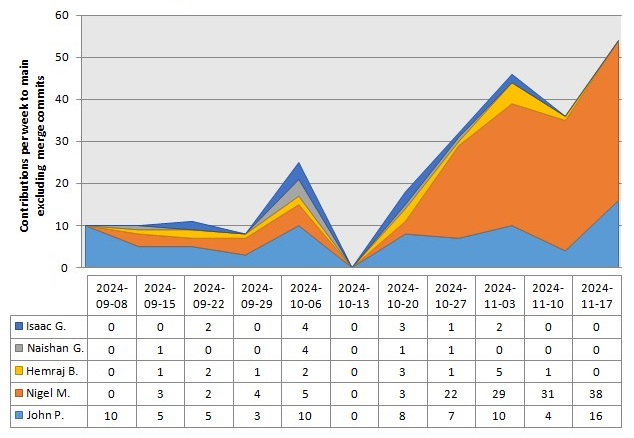
\includegraphics{2024-11-24_contributions}}
\end{figure}


\newpage
\section{Issue Tracker}

% \wss{For each team member how many issues have they authored (including open and closed issues (O+C)) and how many have they been assigned (only counting closed issues (C only)) over the time period of interest.}

Total Authored refers to all internal issues authored including features, bugs, documentation, and team meetings/lectures, which are tracked as issues.\\
- "is:issue author:John-Popovici"\\
% is:issue author:John-Popovici
% is:issue author:nigelmoses32
% is:issue author:STARS952
% is:issue author:Isaac020717
% is:issue author:HemrajB87

\noindent
Assigned closed are those issues that have been closed by the specific student.\\
- "is:issue is:closed assignee:John-Popovici"\\
% is:issue is:closed assignee:John-Popovici 
% is:issue is:closed assignee:nigelmoses32
% is:issue is:closed assignee:STARS952
% is:issue is:closed assignee:Isaac020717
% is:issue is:closed assignee:HemrajB87

\noindent
External Authored refers to issues that have been authored in external repositories for the purposes of peer reviews.\\
- found in \url{https://github.com/simon-0215/UNO-Flip-3D/issues}\\

\noindent
In the first column, External as a student refers to those external to our group that have authored issues through peer review.\\
- "is:issue Peer Review in:title"\\


\begin{table}[H]
\centering
\begin{tabular}{lllll}
\toprule
\textbf{ } & \textbf{Total} & \textbf{Assigned} & \textbf{External}\\
\textbf{Student} & \textbf{Authored} & \textbf{Closed} & \textbf{Authored}\\
\midrule
Total & 105 & 50 & 21 \\
\midrule
External & 15 & - & - \\
John P. & 53 & 28 & 21 \\
Nigel M. & 37 & 23 & 0 \\
Naishan G. & 0 & 0 & 0 \\
Isaac G. & 0 & 0 & 0 \\
Hemraj B. & 0 & 1 & 0 \\
\bottomrule
\end{tabular}
\end{table}

% \wss{If needed, an explanation for the counts can be provided here.}
Some issues are closed and marked as having been worked on by two or more assignees, so the sum may not match up exactly to the total.


\newpage
\section{CICD}

Given that our team is developing a Godot video game, the visual and interactive nature of our project makes full CI/CD integration somewhat challenging since there is a need for graphical testing and user input simulations, which standard pipelines don’t readily support. Instead, we will focus on integrating Continuous Integration practices that focus on code consistency and collaboration.

Our team will use CI to automate build processes, to ensure that each new feature or fix is integrated into the latest codebase. And we can also implement CI to run unit tests on core game logic/backend systems, to ensure that critical functionalities work as expected with each update. This approach makes the most of the advantages of CI/CD while still most closely adhering to the needs and limitations of our specific project.

\end{document}
